%Chapter 10
\chapter{Final result}
ECG-ira (ECG instant rapid analyzer) is a fully working mobile software application able to replace and fulfill most of the functionalities of an analog desktop application. The solution was designed according to the best mobile application development principles and it resulted working fine on all the smartphones\cite{ref27} we tested it on. In this chapter we will show the final results providing significant screenshots of the application and metrics related to the performances evaluated and calculated with the application running on different devices.
\section{App Screens}
By launching the application the first screen is the home screen. It is the starting point, here the user can create a new record (starting a new acquisition with the ZEcg device), he can open the list of records (previously acquired or already present in the device system folder), he can discover and establish  a connection with an acquisition device for future acquisitions and he can access to the application settings section where he can customize the application behaviour and tune some settings like the default folder to store in and open the records from.
\begin{figure}[ht!]
	\centering
	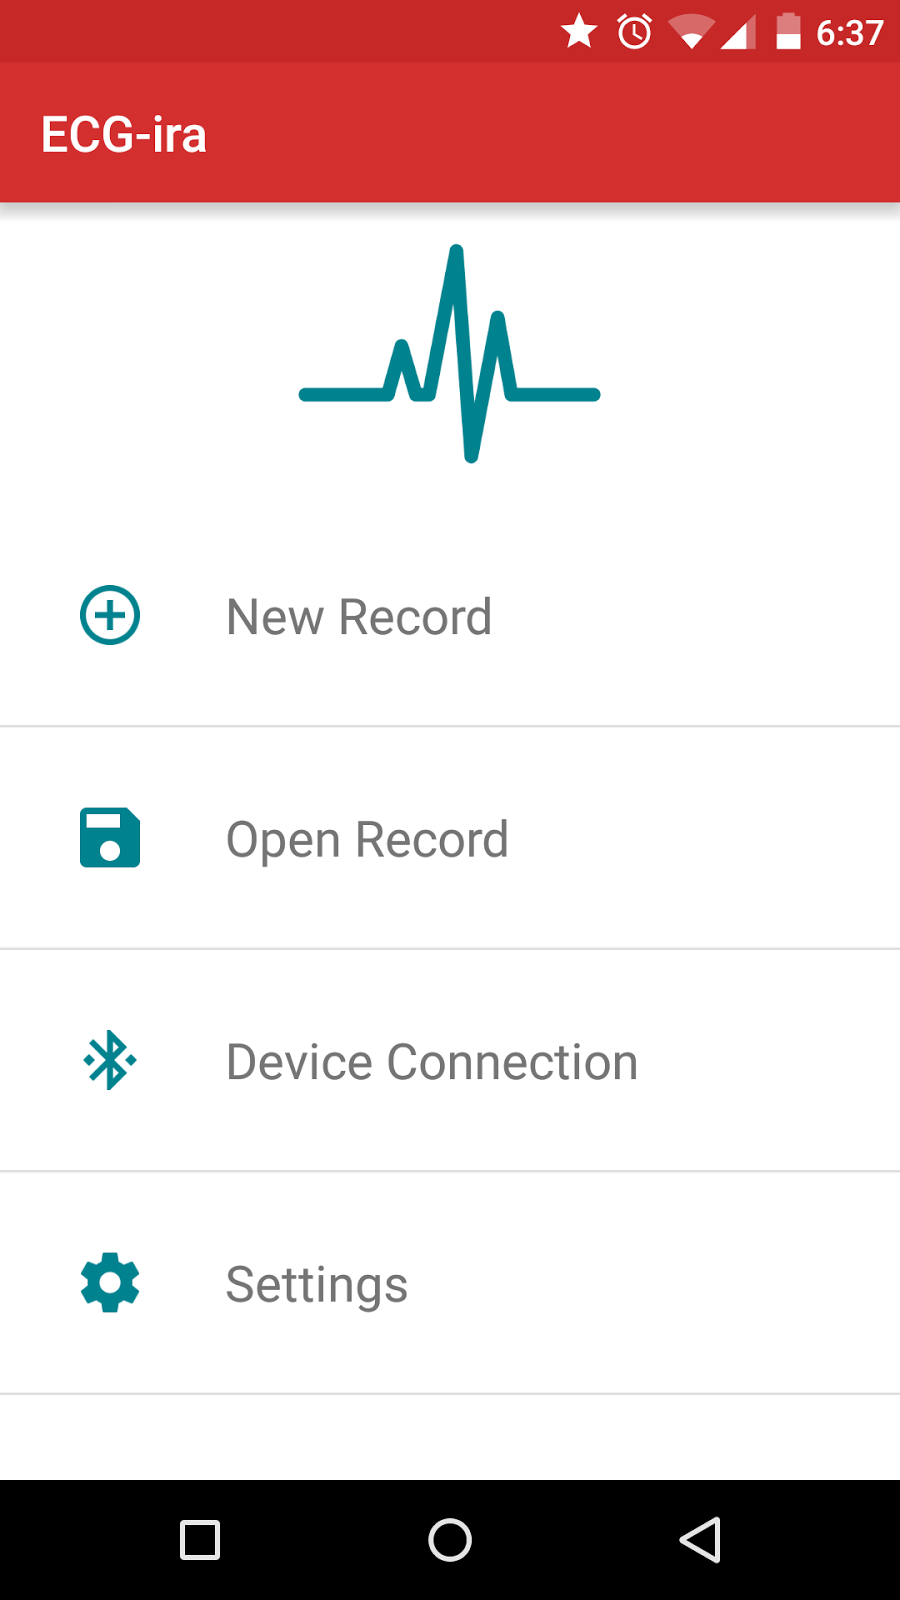
\includegraphics[width=90mm]{figures/ch10/1.png}
	\caption{The home screen of the application ECG-ira.}
	\label{fig10.1}
\end{figure}
\begin{SCfigure}
	\centering
	\caption{The form to be compiled before a record can start. It is necessary to bind any record to a patient data in order to avoid confusion between ecg records. This data is also useful for a fully understanding of the record itself.}
	\includegraphics[width=0.6\textwidth]%
	{figures/ch10/1.png}
	\label{fig10.2}
\end{SCfigure}